\section{Résultat}

Dans la première étude, on fait varier le nombre de colonnes du plateau en conservant un nombre constant de lignes (20) et de pac-mans (2). Pour chaque taille de plateau donnée, on récupère le nombre de pas de temps pour 6 \textit{seeds} différents afin de faire une moyenne. On remarque qu’en augmentant, la taille du plateau a tendance à faire augmenter le temps nécessaire aux pac-mans pour manger tous les fruits. Cela pouvait être plutôt prévisible car en augmentant la taille du plateau les fruits ont de fortes chances de se retrouver plus loin des pacmans à l’initialisation.
En augmentant le nombre de tests avec des seeds différents et des tailles encore plus grandes on aurait pu avoir une courbe de tendance plus précise qui pourrait peut-être nous donner la relation entre la taille du plateau et le temps de résolution.

\begin{figure}[H]
	\centering
	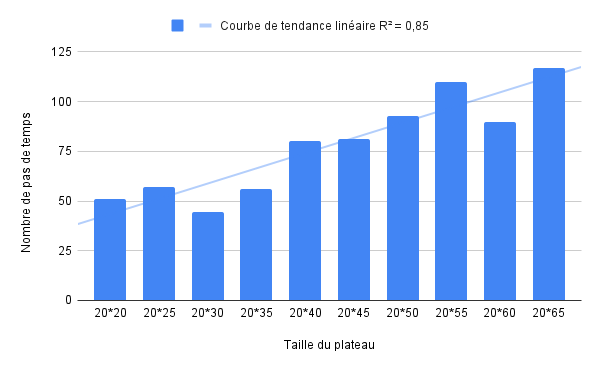
\includegraphics[width=0.8\textwidth]{image/resultat1}
	\caption{Nombre de pas de temps en fonction de la taille du plateau}
\end{figure}

Pour la seconde étude, on fait varier le nombre de pacmans en conservant une taille constante pour le plateau, 20*20. Cette taille a été choisie car elle permet de ne pas avoir un temps de calcul trop long au-delà de 4 robots. 5 plateaux différents ont été testés en faisant varier le nombre de pacmans. On ne peut pas voir directement de lien entre le temps mis par les pacmans pour manger tous les fruits et le nombre de pacmans. Cela est certainement dû au fait que le nombre de fruits est le même que le nombre de pacmans et qu'ils ne sont pas placés de façon aléatoire, donc leur nombre augmentent en même temps dans les tests. Ici aussi, des tests avec un plus grand nombre de plateaux et avec des nombres de pacmans plus grands auraient potentiellement pû permettre d’établir un lien entre les deux données mises en jeu. Une amélioration de notre système pourrait être dans le futur de décorrelé le nombre d'objectifs et le nombre d'agents
\begin{figure}[H]
	\centering
	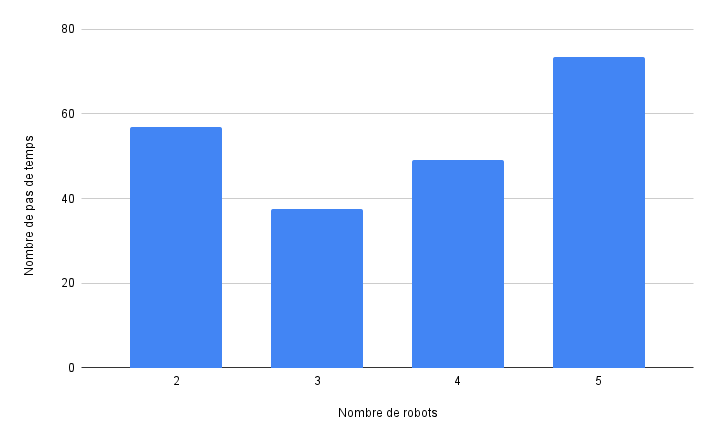
\includegraphics[width=0.8\textwidth]{image/resultat2}
	\caption{Nombre de pas de temps en fonction du nombre de robots}
\end{figure}
